\begin{frame}
\begin{example}[Find the length of the arc of $y = \frac{1}{6}e^{3x} + \frac{1}{6} e^{ -3x}$ from $x = 0$ to $x = 1$.]
\begin{columns}
\column{0.15\textwidth}

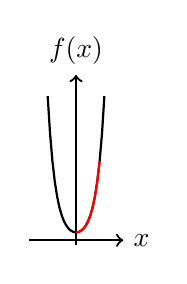
\begin{tikzpicture}[scale=.3,domain=-1.5:1.5]
  %\draw[very thin,color=gray] (-0.1,-1.1) grid (3.9,3.9);
  \draw[thick, ->] (-2,0) -- (2,0) node[right] {$x$};
  \draw[thick, ->] (0,-.2) -- (0,7) node[above] {$f(x)$};
  \draw[thick, domain=-1.2:1.2] plot (\x, {exp(3*\x)/6+exp(-3*\x)/6});
\draw[thick,color=red, domain=0:1] plot (\x, {exp(3*\x)/6+exp(-3*\x)/6});
\end{tikzpicture}


\column{0.85\textwidth}

%\abovedisplayskip=0pt
%\belowdisplayskip=0pt
%\abovedisplayshortskip=0pt
%\belowdisplayshortskip=0pt
\begin{align*}
\uncover<2->{\alert<handout:0| 2-3>{y'}} %
& \uncover<2->{\alert<handout:0| 2-3>{=}}  %
\uncover<3->{\alert<handout:0| 3>{\frac{1}{2}e^{3x} - \frac{1}{2}e^{-3x}}.} \\%
& \uncover<4->{=}  %
\uncover<4->{a-b \textrm{ where } a = \frac{1}{2}e^{3x}, b = \frac{1}{2}e^{-3x}, \textrm{ and } 2ab=\frac12\\}%
\uncover<5->{L} %
& \uncover<5->{=}  %
\uncover<5->{\int_0^1 \sqrt{1 + (y')^2} \diff x} %
 \uncover<6->{=} 
\uncover<6->{\int_0^1 \sqrt{\left( \frac{1}{2}e^{3x} + \frac{1}{2}e^{-3x}\right)^2} \diff x} \\%
& \uncover<7->{=}  %
\uncover<7->{\int_0^1 \left( \alert<handout:0| 8-9>{\frac{1}{2}e^{3x}} + \alert<handout:0| 10-11>{\frac{1}{2}e^{-3x}}\right) \diff x} %
 \uncover<8->{=}  %
\uncover<8->{{\left[ \uncover<9->{\alert<handout:0| 9>{\frac{1}{6}e^{3x}}} \uncover<11->{\alert<handout:0| 11>{- \frac{1}{6}e^{-3x}}}\right]}^1_0} %
 \uncover<12->{=}  %
\uncover<12->{\frac{ e^3 - e^{-3}}{6}.} %
\end{align*}
\end{columns}
\end{example}
\end{frame}
% end module arc-length-half-ex






